For one dimensional data, the evaluation covers the following tasks:

\begin{itemize}
	\item Find a structure for recursive model index empirically.
	\item Compares the performance between baseline model, recursive model and traditional B-Tree.
\end{itemize}

\subsection{Dataset}

For one dimensional case, we manually generate two columns of the data:

\begin{itemize}
	\item The first column contains the keys $X$, which is randomly sampled from a given distribution.
	\item Then we assign the keys into different pages according to a preset parameter $N_{page}$ for page size. Specifically, the first $N_{page}$ keys will be assigned to the first page, the second $N_{page}$ keys will be assigned to the second page and so on so forth. After the assignments, we set the second column $Y$ to be the page index of the corresponding $x$.
\end{itemize}

\begin{figure}
    \centering
    \begin{subfigure}[b]{0.3\textwidth}
    	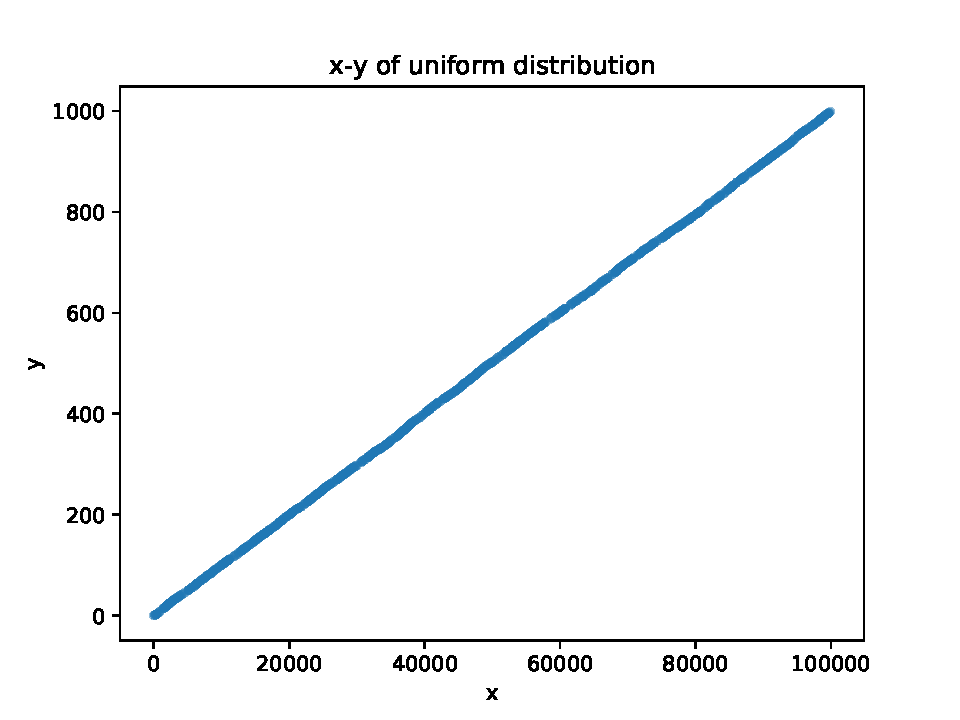
\includegraphics[width=\textwidth]{graphs/evaluation/uniform.pdf}
    	\caption{Uniform}
    \end{subfigure}
    \hfill
	\begin{subfigure}[b]{0.3\textwidth}
    	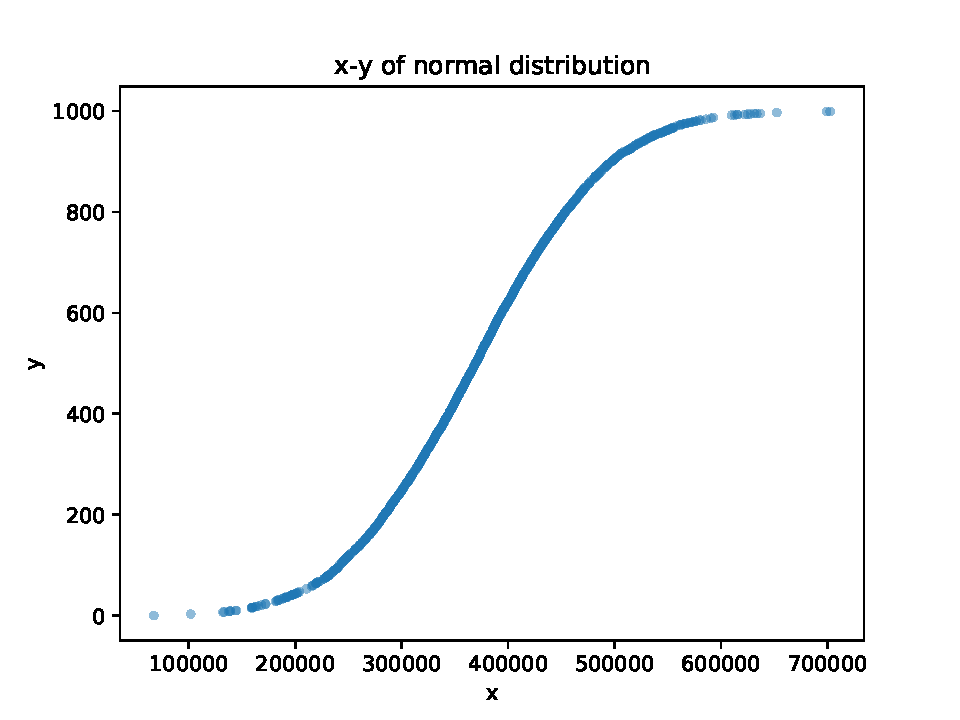
\includegraphics[width=\textwidth]{graphs/evaluation/normal.pdf}
    	\caption{Normal}
    \end{subfigure}
    \hfill
    \begin{subfigure}[b]{0.3\textwidth}
    	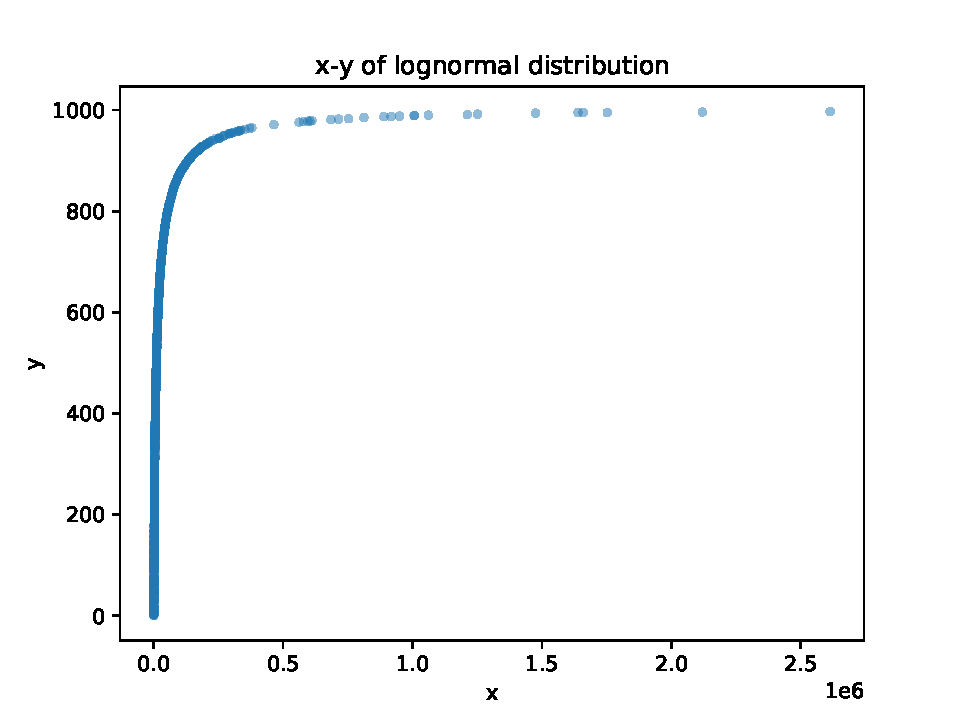
\includegraphics[width=\textwidth]{graphs/evaluation/lognormal.pdf}
    	\caption{Lognormal}
    \end{subfigure}
    \caption{The x-y graph where x is randomly sampled from a certain distribution}
    \label{fig:dist_x_y}
\end{figure}

\subsection{Hyper-Parameter Searching}

We first generate $10,000$ data points where $X$ is from a lognormal distribution $\text{Lognormal}(0, 4)$. In the Fig \ref{fig:dist_x_y}, we illustrate the $x-y$ relations where $X$ is randomly sampled from a uniform, normal or lognormal distribution.

We use three groups to find the best recursive model for lognormal data.
\begin{itemize}
	\item All models are fully connected neural networks. The numbers of second-level models are $200, 400,$ and $600$ respectively. The numbers of third-level models are $2000, 4000$ and $6000$ for each number of second-level models.
	\item All models are linear regression models. The number of second-level models are $200, 400,$ and $600$ respectively. The number of third-level models are $2000, 4000$ and $6000$ for each number of second-level models.
	\item Models are combinations of fully connected neural networks and linear regression models. The numbers of second-level and third-level models are determined by the best settings in the previous two group.
\end{itemize}

\begin{figure}
	\begin{tikzpicture}[font=\small]
	\pgfplotsset{%
		width=0.55\textwidth,
		height=0.60\textwidth,
		minor grid style = {dotted},
	}
	\tikzstyle{every node}=[font=\footnotesize]
	\begin{groupplot}[group style={
                  group name=firstplot,
                  group size= 2 by 2}]
    
    \nextgroupplot[title=Group 1 (Fully Connected Network),
			xbar,
			y axis line style = { opacity = 0 },
			axis x line= none,
			ytick             = data,
			tickwidth = 0pt,
			enlarge y limits  = 0.1,
			enlarge x limits  = 0.5,
			symbolic y coords = {600+6000, 600+4000, 600+2000, 400+6000, 400+4000, 400+2000, 200+6000, 200+4000, 200+2000},
			nodes near coords]
    \addplot coordinates { 
		    (653.8536667,200+2000)
			(1.134166667,200+4000)
			(196.9116667,200+6000)
			(113246.196,400+2000) 
			(113652.3212,400+4000)
			(51.00183333,400+6000)
			(113246.2647,600+2000)
			(18.99766667,600+4000)
			(142041.6877,600+6000)};
	\label{plots:mse}
	
    \addplot coordinates { 
		    (7487.059896,200+2000)
			(24440.75523,200+4000)
			(13034.22656,200+6000)
			(9208.992183,400+2000)
			(12695.55731,400+4000)
			(15434.78905,400+6000)
			(9745.335942,600+2000)
			(20434.90626,600+4000)
			(8118.023442,600+6000)};
	\label{plots:memory}
	
    \nextgroupplot[title=Group 2 (Linear Regression),
			xbar,
			y axis line style = { opacity = 0 },
			axis x line= none,
			ytick=\empty,
			tickwidth = 0pt,
			enlarge y limits  = 0.1,
			enlarge x limits  = 0.5,
			symbolic y coords = {600+6000, 600+4000, 600+2000, 400+6000, 400+4000, 400+2000, 200+6000, 200+4000, 200+2000},
			nodes near coords]
     \addplot coordinates { 
		    (8246.633985,200+2000)
			(7326.238372,200+4000)
			(6276.09111,200+6000)
			(120427.9247,400+2000)
			(6783.428749,400+4000)
			(5998.720313,400+6000)
			(121932.5051,600+2000)
			(8434.091306,600+4000)
			(35342.6365,600+6000)};
     \addplot coordinates { 
		    (4348.463542,200+2000)
			(18769.81252,200+4000)
			(13297.72135,200+6000)
			(5143.059892,400+2000)
			(12864.80731,400+4000)
			(8041.416654,400+6000)
			(4986.927088,600+2000)
			(13843.60678,600+4000)
			(8366.570317,600+6000)};
	\coordinate (top) at (rel axis cs:0,1);
	
    \nextgroupplot[title=Group 3 (Hybrid),
			xbar,
			y axis line style = { opacity = 0 },
			axis x line= none,
			ytick             = data,
			tickwidth = 0pt,
			enlarge y limits  = 0.1,
			enlarge x limits  = 0.5,
			symbolic y coords = {FCN/LR/FCN, LR/FCN/LR, FCN/LR/LR, FCN/FCN/LR, LR/FCN/FCN, LR/LR/FCN},
			nodes near coords]
    \addplot coordinates { 
		    (14478.05283,LR/LR/FCN)
			(13656.1507,LR/FCN/FCN)
			(12191.8397,FCN/FCN/LR)
			(13403.64758,FCN/LR/LR) 
			(12567.93278,LR/FCN/LR)
			(11572.93555,FCN/LR/FCN)};
    \addplot coordinates { 
		    (220.4973958,LR/LR/FCN)
			(9318.697933,LR/FCN/FCN)
			(602.2005208,FCN/FCN/LR)
			(5229.914058,FCN/LR/LR) 
			(6588.58335,LR/FCN/LR)
			(8292.059883,FCN/LR/FCN)};
	\coordinate (bot) at (rel axis cs:1,0);
	
    \end{groupplot}

	\path (top|-current bounding box.south)--
	  coordinate(legendpos)
	  (bot|-current bounding box.east);
	\matrix[
		matrix of nodes,
		anchor=south,
		draw,
		inner sep=0.2em,
		draw
		]at([xshift=20ex]legendpos)
		{
		\ref{plots:mse}& Mean Square Error \\
		\ref{plots:memory}& Memory Usage (KB)\\
	};
\end{tikzpicture}
\end{figure}

From the experiment results, we found that the second setting in group 1 (1 FCN model as root, 200 FCN models as second-level models and 4000 FCN models as third-level models) is the best regarding the mean square error. We also have the following findings in this searching process.

\begin{itemize}
	\item Generally, the average error in the group $1$, where all models are fully connected neural networks, is less than the error in the group $2$. We conclude that the fully connected neural networks have the potential to be more accurate, i.e. it could achieve a small error if we tuned the parameters properly.
	\item Tuning a model is tedious and can be costly. There are lots of hyper-parameters to choose from, such as the number of models in each level, types of models in each level, number of levels, and the internal hyper-parameters in each model. Using grid search, as we did in this experiment, can be costly and time-consuming.
\end{itemize}

\subsection{Comparisons across Distributions}

After the search process for a recursive model, we then conduct experiments on several different distributions and sizes datasets. During this process, we use the following settings:

\begin{itemize}
	\item The $\boldsymbol{X}$ is generated from \textit{uniform}, \textit{normal} and \textit{lognormal} distribution.
	\item For each distribution, we generate $1$ thousand, $10$ thousand, $100$ thousand and $1$ million data points. We then assign the generated data points into pages where $N_{page}=10$.
	\item We use a B-Tree with degree=$20$, a fully connected neural network with two layers and 32 nodes per layer, and a recursive model with 200 second-layer models and 4000 third-layer models.
\end{itemize}

We compare the following performance metrics:

\begin{itemize}
	\item The query time per key and the memory usage among three index models.
	\item The mean square error caused by the fully connected network and the recursive model across different distributions.
	\item The construction time among three index models.
\end{itemize}

\begin{figure}
 \centering
     \begin{subfigure}[b]{0.28\textwidth}
         \centering
         \begin{tikzpicture}[font=\small]
	\pgfplotsset{compat=1.10, width=\textwidth, height=\textwidth}
	\begin{axis}[
		xmode=log,
		axis y line*=left,
		xlabel=Number of datapoints,
		ylabel=Average Query time,
		xtick={1000,10000,100000,1000000},
	]
	\addplot[smooth, mark=x, blue]
	coordinates{
		(1000, 4.93824E-05)
		(10000, 6.10835E-05)
		(100000, 6.41705E-05)
		(1000000, 6.67412E-05)
	}; \label{plot_one}
	\end{axis}
	
	\begin{axis}[
		xmode=log,
  		axis y line*=right,
  		axis x line=none,
 	  	ylabel=Memory Usage,
 	  	xtick={1000,10000,100000,1000000},
	]
	\addplot[smooth,mark=o,red]
  	coordinates{
    	(1000,444.0729167)
    	(10000,4417.733333)
    	(100000,44146)
    	(1000000,442610.6667)
	};
	\end{axis}	
\end{tikzpicture}
         \caption{B-Tree}
         \label{fig:exp2_1_btree}
     \end{subfigure}
     \hfill
     \begin{subfigure}[b]{0.28\textwidth}
         \centering
         \begin{tikzpicture}[font=\small]
	\pgfplotsset{compat=1.10, width=\textwidth, height=\textwidth}
	\begin{axis}[
		xmode=log,
		axis y line*=left,
		xlabel=Number of datapoints,
		ylabel=Average Query time (ms),
		xtick={1000,10000,100000,1000000},
	]
	\addplot[smooth, mark=x, blue]
	coordinates{
		(1000, 0.136657)
		(10000, 0.119728)
		(100000, 0.11154)
		(1000000, 0.137276)
	}; \label{plot_one}
	\end{axis}
	
	\begin{axis}[
		xmode=log,
  		axis y line*=right,
  		axis x line=none,
 	  	ylabel=Memory Usage,
 	  	xtick={1000,10000,100000,1000000},
	]
	\addplot[smooth,mark=o,red]
  	coordinates{
    	(1000,28.515625)
    	(10000,28.515625)
    	(100000,28.515625)
    	(1000000,28.515625)
	};
	\end{axis}	
\end{tikzpicture}
         \caption{FCN}
         \label{fig:exp2_1_fcn}
     \end{subfigure}
     \hfill
     \begin{subfigure}[b]{0.28\textwidth}
         \centering
         \begin{tikzpicture}[font=\small]
	\pgfplotsset{compat=1.10, width=\textwidth, height=\textwidth}
	\begin{axis}[
		xmode=log,
		axis y line*=left,
		xlabel=Number of datapoints,
		ylabel=Average Query time (ms),
		xtick={1000,10000,100000,1000000},
	]
	\addplot[smooth, mark=x, blue]
	coordinates{
		(1000, 0.279265)
		(10000, 0.272018)
		(100000, 0.255443)
		(1000000, 0.325924)
	}; \label{plot_one}
	\end{axis}
	
	\begin{axis}[
		xmode=log,
  		axis y line*=right,
  		axis x line=none,
 	  	ylabel=Memory Usage,
 	  	xtick={1000,10000,100000,1000000},
	]
	\addplot[smooth,mark=o,red]
  	coordinates{
    	(1000,4666.032118)
    	(10000,21933.81598)
    	(100000,15421.51737)
    	(1000000,16624.75696)
	};
	\end{axis}	
\end{tikzpicture}
         \caption{Recursive Model}
         \label{fig:exp2_1_rmi}
     \end{subfigure}
        \caption{The relations between the number of data points, average query time and the memory usage among three different indexes. The blue line represents the average query time and the red line represents the memory usage}
        \label{fig:exp2_1}
\end{figure}

\begin{mscconclusion}
	From Fig \ref{fig:exp2_1}, we analyse the time complexities for query and the space complexity for storing three different index models.
	
	\begin{enumerate}
	\item From Fig \ref{fig:exp2_1_btree}, we verified that the average query time per key for a B-Tree is growing as the number of data points is increasing. It grows with a complexity of $\mathcal{O}(\log n)$, i.e. it grows slower when there are more data points. 
	\item From Fig \ref{fig:exp2_1_fcn}, we found that the memory usage of a fully connected neural network is significantly less than the memory usage of B-Tree. Meanwhile, the fully connected neural network takes constant memory usage, as there is a fixed number of nodes in the neural network. Similarly, the average query time is also a constant in theory. In the experiments, the average query time is changing but likely caused by turbulence.
	\item From Fig \ref{fig:exp2_1_rmi}, we found that the memory usage of a recursive model is significantly higher than the memory usage of a fully connected neural network, but still less than a B-Tree, which is because the recursive model consists of thousands fully connected network. The memory usage of a recursive model is fluctuating, as the actually used number of the fully connected network varies. The query time is higher than B-Tree and single fully connected network, but still a constant in theory, as there is only a fixed number of computations.
	\end{enumerate}
\end{mscconclusion}

\begin{figure}
 \centering
     \begin{subfigure}[b]{0.3\textwidth}
         \centering
         \begin{tikzpicture}[font=\small]
	\pgfplotsset{compat=1.10, width=\textwidth, height=\textwidth}
	\begin{axis}[
		xmode=log,
		ymode=log,
		xlabel=Number of datapoints,
		ylabel=Mean Square Error,
		xtick={1000,10000,100000,1000000},
	]
	\addplot[smooth, mark=x, blue]
	coordinates{
		(1000, 0.275)
		(10000, 1.505166667)
		(100000, 12.26908333)
		(1000000, 136.2974717)
	};
	\addplot[smooth,mark=o,red]
  	coordinates{
    	(1000,0.113333333)
    	(10000,0.105333333)
    	(100000,38.88833333)
    	(1000000,6438.175392)
	};
	\end{axis}
\end{tikzpicture}
         \caption{Uniform}
         \label{fig:exp2_2_uniform}
     \end{subfigure}
     \hfill
     \begin{subfigure}[b]{0.3\textwidth}
         \centering
         \begin{tikzpicture}[font=\small]
	\pgfplotsset{compat=1.10, width=\textwidth, height=\textwidth}
	\begin{axis}[
		xmode=log,
		ymode=log,
		xlabel=Number of datapoints,
		ylabel=Mean Square Error,
		xtick={1000,10000,100000,1000000},
	]
	\addplot[smooth, mark=x, blue]
	coordinates{
		(1000, 0.315)
		(10000, 4.399333333)
		(100000, 38.88833333)
		(1000000, 1268107500)
	};
	\addplot[smooth,mark=o,red]
  	coordinates{
    	(1000,0.106666667)
    	(10000,1.807833333)
    	(100000,11199.25468)
    	(1000000,18790922.95)
	};
	\end{axis}
\end{tikzpicture}
         \caption{Normal}
         \label{fig:exp2_2_normal}
     \end{subfigure}
     \hfill
     \begin{subfigure}[b]{0.3\textwidth}
         \centering
         \begin{tikzpicture}[font=\small]
	\pgfplotsset{compat=1.10, width=\textwidth, height=\textwidth}
	\begin{axis}[
		xmode=log,
		ymode=log,
		xlabel=Number of datapoints,
		ylabel=Mean Square Error,
		xtick={1000,10000,100000,1000000},
	]
	\addplot[smooth, mark=x, blue]
	coordinates{
		(1000, 0.426666667)
		(10000, 83771.87783)
		(100000, 16752181)
		(1000000, 1675484449)
	};
	\addplot[smooth,mark=o,red]
  	coordinates{
    	(1000,0.108333333)
    	(10000,30089.25283)
    	(100000,831226.3517)
    	(1000000,1611797.93)
	};
	\end{axis}
\end{tikzpicture}
         \caption{Lognormal}
         \label{fig:exp2_2_lognormal}
     \end{subfigure}
        \caption{The relations between the number of data points and the mean square error in three different distributions. The blue line represents the fully connected network and the red line represents the recursive model}
        \label{fig:exp2_2}
\end{figure}

\begin{mscconclusion}
	From Fig \ref{fig:exp2_2}, we analyse the errors of fully connected network and recursive model on several different distributed datasets.
	\begin{enumerate}
		\item From Fig \ref{fig:exp2_2_uniform}, we found that both fully connected neural network and recursive model are capable of modelling uniformly distributed dataset with a rather low error. The fully connected neural network could achieve relatively less error, especially when there is a large amount of data.		
        \item From Fig \ref{fig:exp2_2_normal}, we found that the error is increasing exponentially as the number of data points is increasing. The error in the fully connected neural network is significantly higher than the recursive model.
		\item From Fig \ref{fig:exp2_2_lognormal}, we found that the error from the recursive model is significantly less than the error in the fully connected neural network. Combined with \ref{fig:exp2_2_normal} and \ref{fig:exp2_2_uniform}, we conclude that the recursive model could surpass fully connected network when the data is not uniformly distributed. That means the fully connected network is suitable for uniformly distributed data. We will analyse this property in more detail in the chapter \textit{Insights and Findings}.
	\end{enumerate}
\end{mscconclusion}

\begin{figure}
 \centering
     \begin{subfigure}[b]{0.3\textwidth}
         \centering
         \begin{tikzpicture}[font=\small]
	\pgfplotsset{compat=1.10, width=\textwidth, height=\textwidth}
	\begin{axis}[
		xmode=log,
		ymode=log,
		xlabel=Number of datapoints,
		ylabel=Construction Time,
		xtick={1000,10000,100000,1000000},
	]
	\addplot[smooth, mark=x, blue]
	coordinates{
		(1000, 0.074044889)
		(10000, 0.798198778)
		(100000, 10.23407889)
		(1000000, 119.5872338)
	};
	\end{axis}
\end{tikzpicture}
         \caption{B-Tree}
         \label{fig:exp2_3_btree}
     \end{subfigure}
     \hfill
     \begin{subfigure}[b]{0.3\textwidth}
         \centering
         \begin{tikzpicture}[font=\small]
	\pgfplotsset{compat=1.10, width=\textwidth, height=\textwidth}
	\begin{axis}[
		xmode=log,
		ymode=log,
		xlabel=Number of datapoints,
		ylabel=Construction Time,
		xtick={1000,10000,100000,1000000},
	]
	\addplot[smooth, mark=x, blue]
	coordinates{
		(1000, 14.20050143)
		(10000, 138.1622851)
		(100000, 1414.916556)
		(1000000, 10198.93739)
	};
	\end{axis}
\end{tikzpicture}
         \caption{FCN}
         \label{fig:exp2_3_fcn}
     \end{subfigure}
     \hfill
     \begin{subfigure}[b]{0.3\textwidth}
         \centering
         \begin{tikzpicture}[font=\small]
	\pgfplotsset{compat=1.10, width=\textwidth, height=\textwidth}
	\begin{axis}[
		xmode=log,
		ymode=log,
		xlabel=Number of datapoints,
		ylabel=Construction Time,
		xtick={1000,10000,100000,1000000},
	]
	\addplot[smooth, mark=x, blue]
	coordinates{
		(1000, 152.3591999)
		(10000, 758.5806553)
		(100000, 1226.519557)
		(1000000, 6418.693972)
	};
	\end{axis}
\end{tikzpicture}
         \caption{Recursive Model}
         \label{fig:exp2_3_rmi}
     \end{subfigure}
        \caption{The relations between the number of data points and the construction time among three different index models.}
        \label{fig:exp2_3}
\end{figure}

\begin{mscconclusion}
	In \ref{fig:exp2_3}, we analyse the construction time of different models.
	\begin{enumerate}
		\item As shown in \ref{fig:exp2_3_btree} and \ref{fig:exp2_3_fcn}, the construction time of both B-Tree and fully connected neural network is increasing almost linearly as the number of data points is increasing. Theoretically, the construction time for B-Tree is $\mathcal{O}(n\log n)$ and $\mathcal{O}(n)$ for fully connected neural network.
		\item In \ref{fig:exp2_3_rmi}, we found that the construction time of recursive model is increasing as well. The time in construction varies by two factors:
			\begin{itemize}
				\item The number of data points will affect the construction time.
				\item As we need to iterate over all possible models in each layer to assign training set, the number of models in each layer will affect the construction time as well.
			\end{itemize}
	\end{enumerate}
\end{mscconclusion}

\subsection{Comparisons on Large Dataset} The last and largest dataset that we used is a large dataset that contains $190$ million key-value pairs that are distributed under lognormal distribution. There are two challenges in this task:

\begin{enumerate}
	\item The training set is too large to be trained and tuned. As our implementation only supports a single process, it would take a tediously long time to train the recursive model.
	\item It takes a super long time (several days in our settings) to evaluate on the very large dataset, as only one CPU thread will be used.
\end{enumerate}

To tackle these challenges, we take the following strategies:

\textbf{Training on Sampled Dataset} We first randomly and uniformed sample from the whole training dataset. By sampling uniformly, we could keep the shape of the distribution unchanged. Assume we sampled $S$ data pairs from the whole training dataset of size $N$, then we define the sampling ratio as $R=\frac{S}{N}$. We then map the output $\tilde{y}$ from our index model to its approximate position by $\hat{y}=\frac{\tilde{y}}{R}$. We illustrate an example in Example 3.\ref{mscexample:sampled_training}.

\begin{mscexample}
	\label{mscexample:sampled_training}
	Assume the \textbf{X} in training set is exponentially distributed as $$[1,2,4,8,16,32,64,128]$$ and we use a sample size $S=4$. As we know the size of the fully training dataset is $N=8$, we have $R=\frac{S}{N}=0.5$. We uniformly sample from the training set and we will get $[1,4,16,64]$. Then we train an index model based on $$[(1,0), (4,1), (16,2), (64,3)]$$ 
	
	For the key $32$ as an example, ideally, we want our index model $\mathcal{F}$ to have an output such that $\tilde{y}=\mathcal{F}(32)=2.5$. Then the original index of the key $32$ can be calculated as $\hat{y}=\frac{\tilde{y}}{R}=\frac{2.5}{0.5}=5$, which is the index of $32$ in the original full training dataset.
\end{mscexample}


\textbf{Evaluation with Multiple Processes} To evaluate our models on the full training set would take several days to complete because there is only one process working on it. As the query is independent of each other, we utilise multiple processes to work on it by taking the following steps:

\begin{enumerate}
	\item We first train our model on the sampled dataset with $S=100,000$.
	\item Then we split the full training set into $10$ pieces such that each piece contains only $19$ million pairs.
	\item Afterwards, we perform the point query with the trained model on each piece in parallel.
	\item Finally, we collect the query time from $10$ pieces and sum them to get the total query time of the full training set. Then we divide it by the number of pairs in total, i.e. $19$ million and get the average query time per key. For the mean square error, we take the average of errors from each piece.
\end{enumerate}

With these two approaches, we achieved the results as shown below:

\begin{table}[h!]
\centering
\begin{tabular}{ |c|c|c|c| }
\hline
Model & Construction Time (s) & Avery Query Time (ms) & Memory Usage (MB)\\ 
\hline
B-Tree (degree=20) & 26356 (1.00x) & \textbf{0.3489 (1.00x)} & 96912 \tablefootnote{The memory usage of each node is larger than previous experiments. It is because the tools for measuring memory usage (\texttt{pympler}) requires extra memory, and caused the program to be killed when there is not enough memory. Hence we use a different tool (\texttt{top}) to measure an approximate memory usage.} \\ 
\hline
Recursive Model & \textbf{334 (0.013x)} & 2.6505 (7.60x) & \textbf{8.836} \\ 
\hline
\end{tabular}
\caption{The construction time, average query time and memory usage of a B-Tree (with a degree=20) and a recursive model.}
\label{exp3}
\end{table}

\begin{mscconclusion}
	From Table \ref{exp3}, we have the following conclusions:
	\begin{enumerate}
		\item The construction time of recursive model can be significantly less than the construction of B-Tree, for two reasons: 
			\begin{itemize}
				\item We sample from the training dataset and avoid iterating over all the data points. In contrast, B-Tree has to iterate all the data points and insert them one by one.
				\item The recursive model trains relatively fast as it can converge in one to a few passes over the data points.
			\end{itemize}
			\item Then average query time for the recursive model is higher than B-Tree, but not significantly higher. The computation costs are mainly on the calculation in fully connected neural networks. The query time for the recursive model can be improved by either using a well-established library, such as PyTorch, that provides faster matrix computation or using faster hardware such as the GPU to improve the query speed.
			\item The memory usage of B-Tree is significantly higher than the recursive model. As we showed above, the memory usage of B-Tree is $\mathcal{O}(n)$ and hence growing linearly. For the recursive model, the memory usage mainly depends on how many models in each layer. Therefore, the memory usage of a recursive model has an upper bound (if all models are used), and then will not grow as the number of data points is growing.
	\end{enumerate}
\end{mscconclusion}









